% ------------------------------------------------------------------------------
% TYPO3 CMS 7.0 - What's New - Chapter "Interfaz de usuario de Backend" (Spanish Version)
%
% @author	Michael Schams <schams.net>
% @author	Michel Mix <mmix@autistici.org>
% @license	Creative Commons BY-NC-SA 3.0
% @link		http://typo3.org/download/release-notes/whats-new/
% @language	Spanish
% ------------------------------------------------------------------------------
% LTXE-CHAPTER-UID:		8f0084cb-89f1e82a-8218b0cc-3688d5de
% LTXE-CHAPTER-NAME:	Interfaz de usuario de Backend
% ------------------------------------------------------------------------------

\section{BackendUI}
\begin{frame}[fragile]
	\frametitle{Interfaz de usuario de Backend}

	\begin{center}\huge{Capítulo 1:}\end{center}
	\begin{center}\huge{\color{typo3darkgrey}\textbf{Interfaz de usuario de Backend}}\end{center}

\end{frame}

% ------------------------------------------------------------------------------
% LTXE-SLIDE-START
% LTXE-SLIDE-UID:		c866406a-f21e0e95-cf86d35a-ad718622
% LTXE-SLIDE-ORIGIN:	fcbdd27c-e9005dff-0f4dd846-000ea412 English
% LTXE-SLIDE-TITLE:		In General
% LTXE-SLIDE-REFERENCE:	https://forge.typo3.org/issues/62333
% LTXE-SLIDE-REFERENCE:	https://forge.typo3.org/issues/62995
% LTXE-SLIDE-REFERENCE:	https://forge.typo3.org/issues/62158
% LTXE-SLIDE-REFERENCE:	https://forge.typo3.org/issues/61454
% ------------------------------------------------------------------------------

\begin{frame}[fragile]
	\frametitle{Interfaz de usuario de Backend}
	\framesubtitle{En general}

	\begin{itemize}
		\item Cambios visuales significativos de la interfaz de usuario Backend
		\item Basado en Twitter Bootstrap versión 3.2.x
		\item Todos los íconos han sido recreados y están en estilo "tile" ahora
		\item Los íconos usan Font Awesome versión 4.2.x
		\item El menú de función izquierdo ha sido ajustado apropiadamente
		\item Los íconos en el menú de función usan en diseño, fondo colorido, pictograma invertido/monocromatico en el primer plano, esquinas redondeadas
		\item El ancho del menú de función puede ser reducido para mostrar sólo los íconos

	\end{itemize}

\end{frame}

% ------------------------------------------------------------------------------
% LTXE-SLIDE-START
% LTXE-SLIDE-UID:		02f1fca9-20458018-f4ac0a60-b67ee9d1
% LTXE-SLIDE-ORIGIN:	0ae980b6-0d2ae6c6-52182f58-aaef69e3 English
% LTXE-SLIDE-TITLE:		Look & Feel (1)
% ------------------------------------------------------------------------------

\begin{frame}[fragile]
	\frametitle{Interfaz de usuario de Backend}
	\framesubtitle{Apariencia \& Función}

	\begin{figure}
		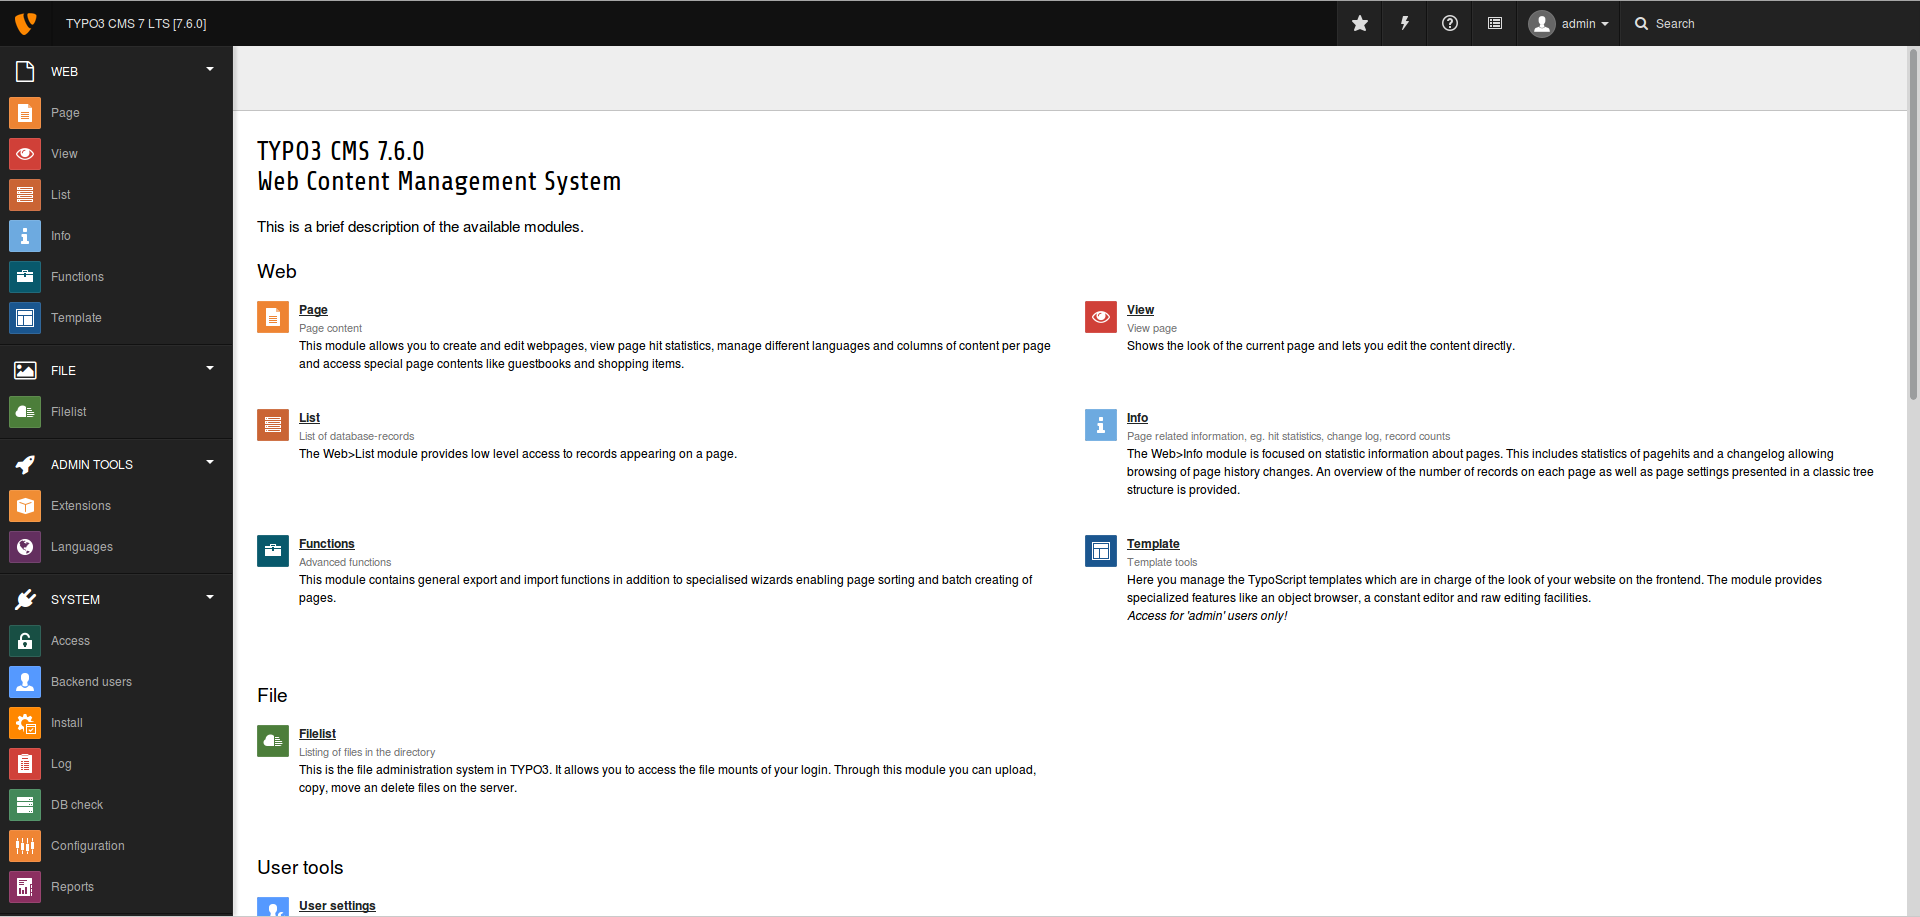
\includegraphics[width=0.90\linewidth]{BackendUserInterface/be-totalscreenshot1.png}
	\end{figure}

\end{frame}

% ------------------------------------------------------------------------------
% LTXE-SLIDE-START
% LTXE-SLIDE-UID:		efee0e82-c2a622af-ed0d8000-ca2758e9
% LTXE-SLIDE-ORIGIN:	250b123b-2c0bfce4-506f16b0-629baa10 English
% LTXE-SLIDE-TITLE:		Look & Feel (2)
% ------------------------------------------------------------------------------

\begin{frame}[fragile]
	\frametitle{Interfaz de usuario de Backend}
	\framesubtitle{Apariencia \& Función}

	\begin{figure}
		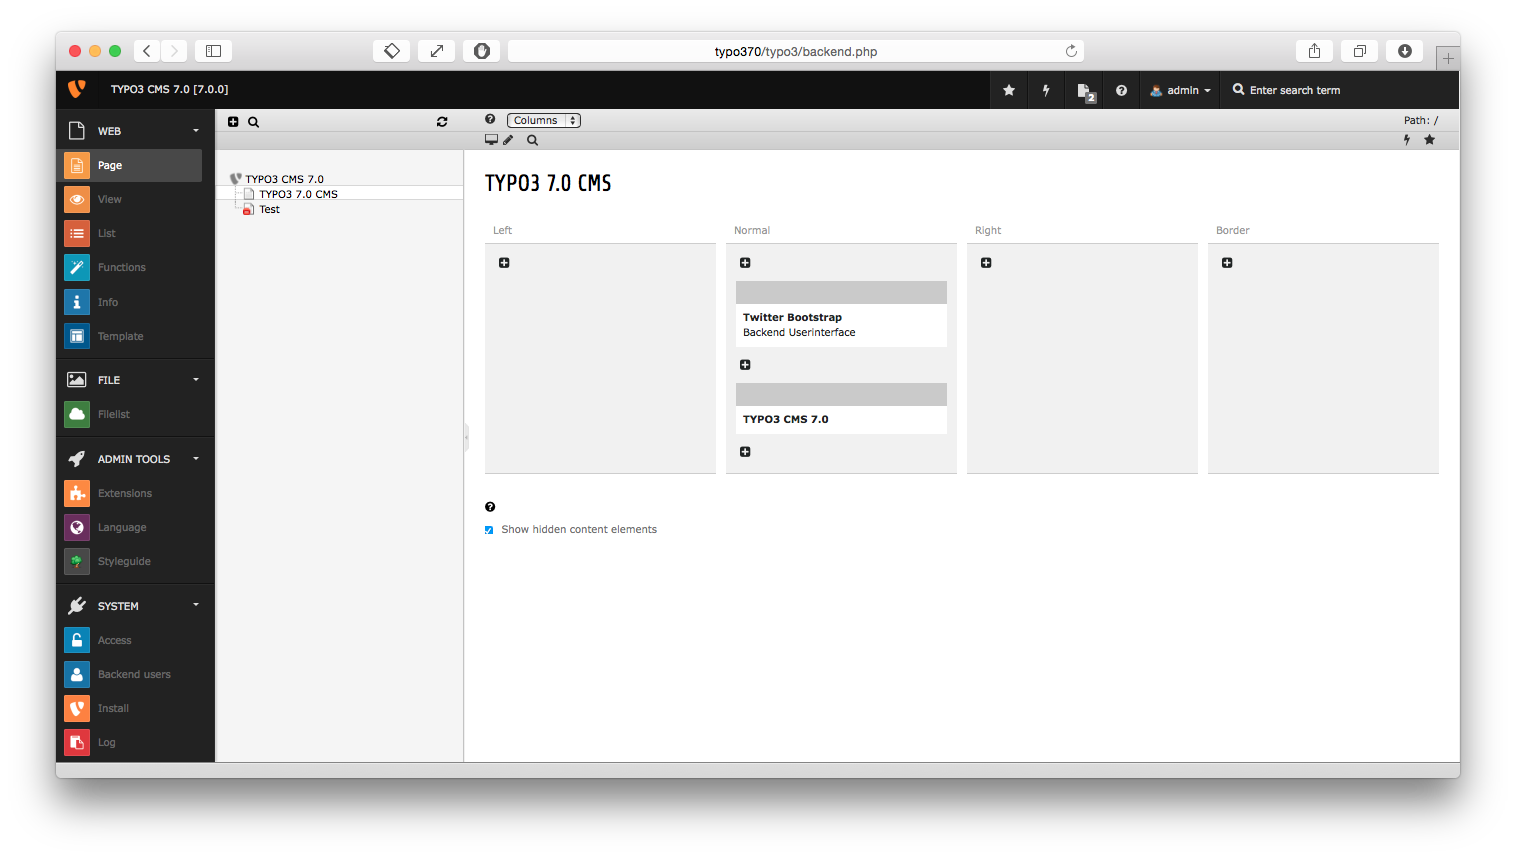
\includegraphics[width=0.90\linewidth]{BackendUserInterface/be-totalscreenshot2.png}
	\end{figure}

\end{frame}

% ------------------------------------------------------------------------------
% LTXE-SLIDE-START
% LTXE-SLIDE-UID:		1f997935-129fb6f1-c73a396a-41882d43
% LTXE-SLIDE-ORIGIN:	2d4d33ee-071ae6ed-9f4d0c04-49361364 English
% LTXE-SLIDE-TITLE:		Look & Feel (3)
% ------------------------------------------------------------------------------

\begin{frame}[fragile]
	\frametitle{Interfaz de usuario de Backend}
	\framesubtitle{Apariencia \& Función}

	\begin{figure}
		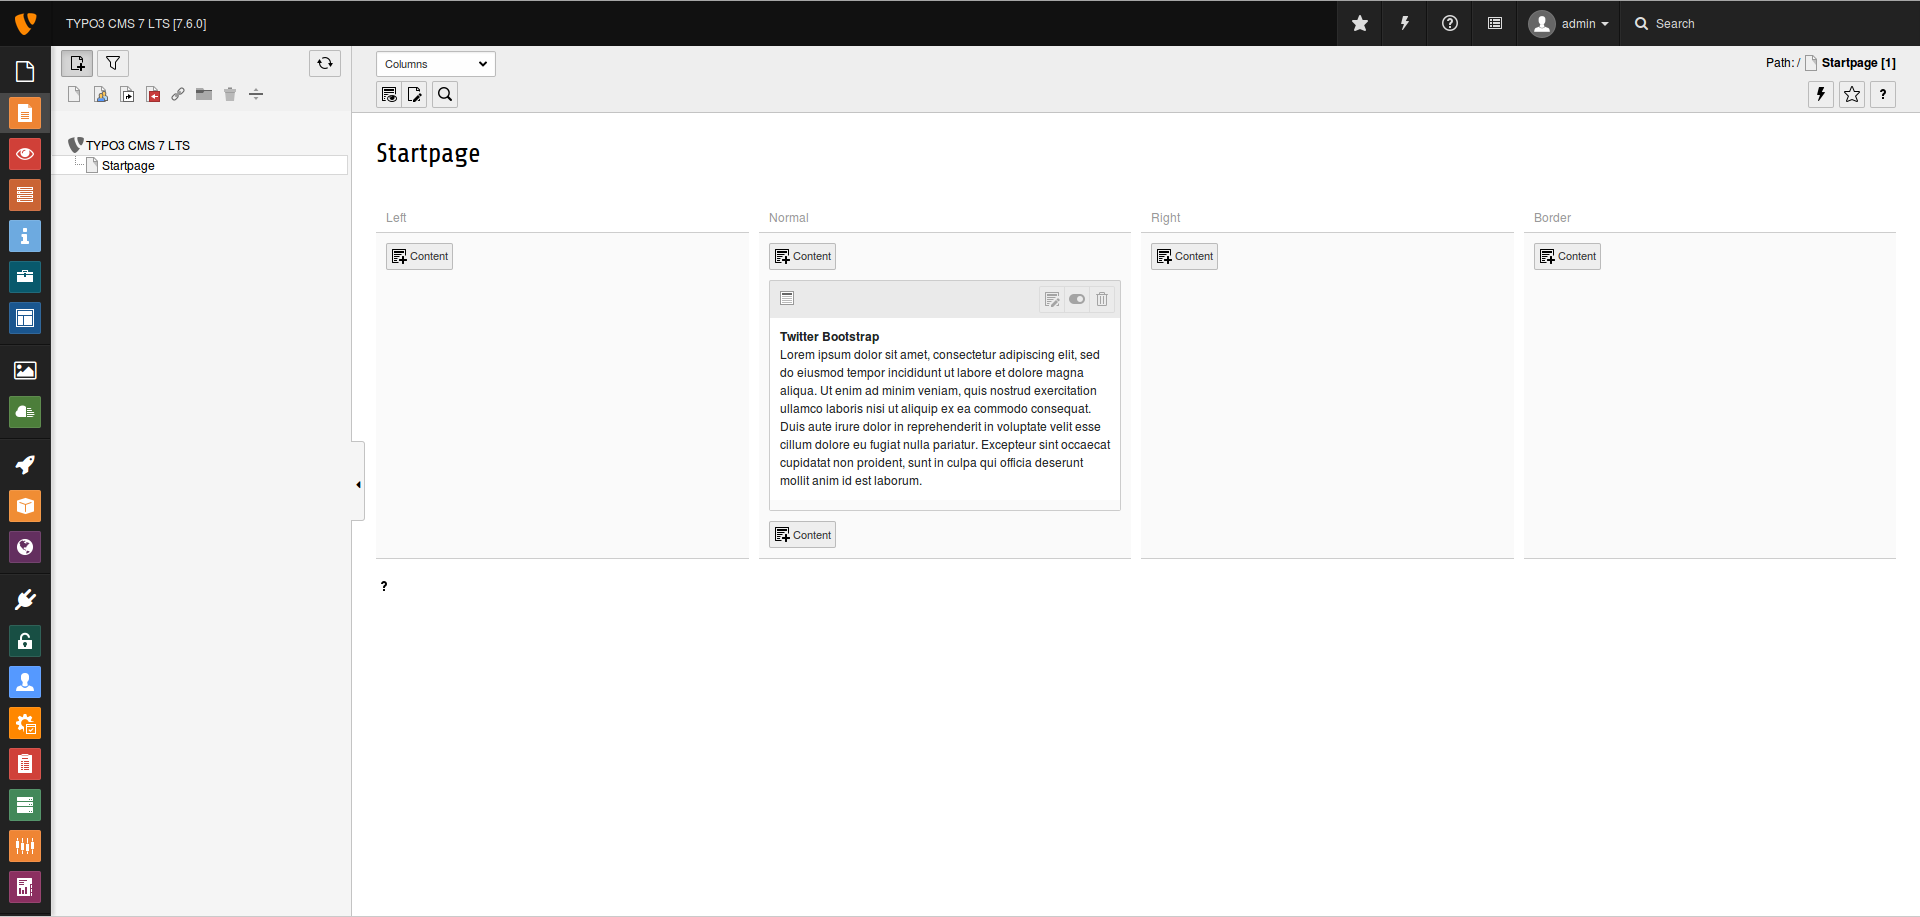
\includegraphics[width=0.90\linewidth]{BackendUserInterface/be-totalscreenshot3.png}
	\end{figure}

\end{frame}

% ------------------------------------------------------------------------------
% LTXE-SLIDE-START
% LTXE-SLIDE-UID:		7a828390-ad90b0af-8dd6c387-4f20dab4
% LTXE-SLIDE-ORIGIN:	de58d070-98483f3d-0949f2d1-856a9e7e English
% LTXE-SLIDE-TITLE:		Backend User Login
% ------------------------------------------------------------------------------

\begin{frame}[fragile]
	\frametitle{Interfaz de usuario de Backend}
	\framesubtitle{Inicio de sesión de usuario de Backend}

	\begin{figure}
		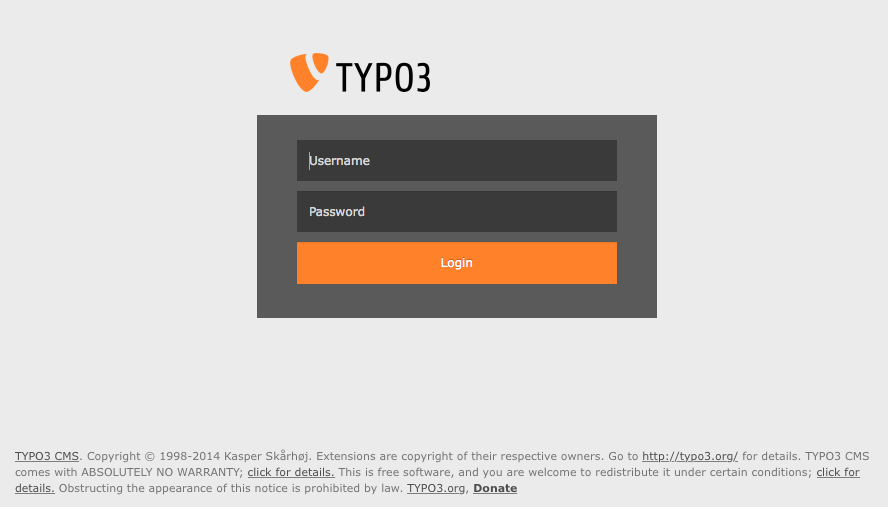
\includegraphics[width=0.80\linewidth]{BackendUserInterface/be-login.png}
	\end{figure}

\end{frame}

% ------------------------------------------------------------------------------
% LTXE-SLIDE-START
% LTXE-SLIDE-UID:		9e2b9f71-e9b46b9a-5ab75175-7c820d2e
% LTXE-SLIDE-ORIGIN:	9baa13c8-78b2f416-28da8e3d-b234e7dc English
% LTXE-SLIDE-TITLE:		Refactor & recolor Modul Menu (Bootstrap)
% LTXE-SLIDE-REFERENCE:	https://forge.typo3.org/issues/62353
% ------------------------------------------------------------------------------

\begin{frame}[fragile]
	\frametitle{Interfaz de usuario de Backend}
	\framesubtitle{Barra superior (Menú de módulo)}

	\begin{figure}
		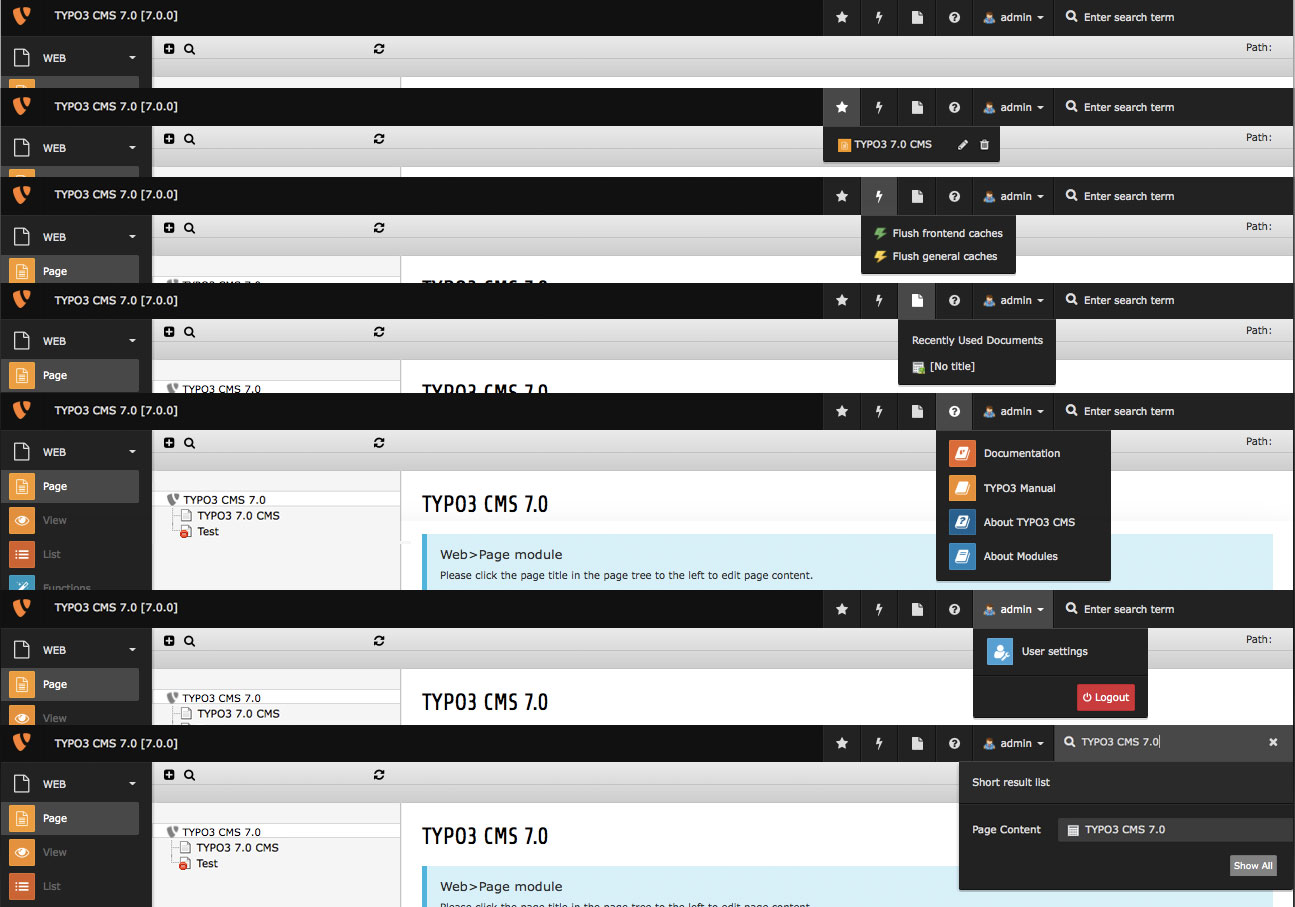
\includegraphics[width=0.70\linewidth]{BackendUserInterface/be-topbar.jpg}
	\end{figure}

\end{frame}

% ------------------------------------------------------------------------------
% LTXE-SLIDE-START
% LTXE-SLIDE-UID:		68ef3249-5a266aab-99abe1f3-cbdbbf5d
% LTXE-SLIDE-ORIGIN:	4369ae5e-948d1afa-8212cd72-c91c660b English
% LTXE-SLIDE-TITLE:		New List Module Styling
% LTXE-SLIDE-REFERENCE:	https://forge.typo3.org/issues/62963
% ------------------------------------------------------------------------------

\begin{frame}[fragile]
	\frametitle{Interfaz de usuario de Backend}
	\framesubtitle{Módulo Lista y Portapapeles}

	\begin{figure}
		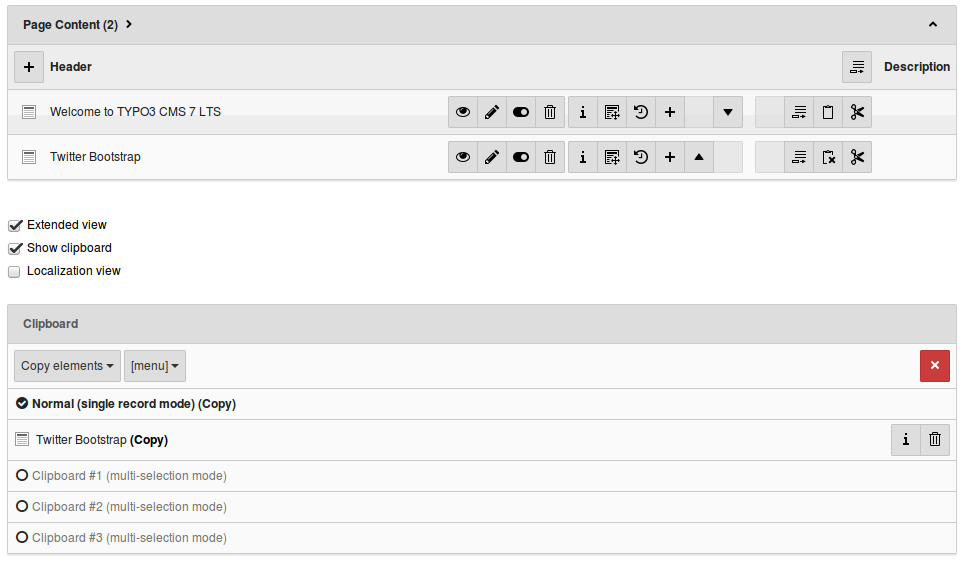
\includegraphics[width=0.80\linewidth]{BackendUserInterface/be-list.png}
	\end{figure}

\end{frame}

% ------------------------------------------------------------------------------
% LTXE-SLIDE-START
% LTXE-SLIDE-UID:		18c5e9bb-d901ccb3-d9d96ca2-3c25b92c
% LTXE-SLIDE-ORIGIN:	252361f7-e5c42ec2-a90ecd64-4331f02b English
% LTXE-SLIDE-TITLE:		Table Style
% LTXE-SLIDE-REFERENCE:	https://forge.typo3.org/issues/62159
% ------------------------------------------------------------------------------

\begin{frame}[fragile]
	\frametitle{Interfaz de usuario de Backend}
	\framesubtitle{Estilo de tabla}

	\begin{figure}
		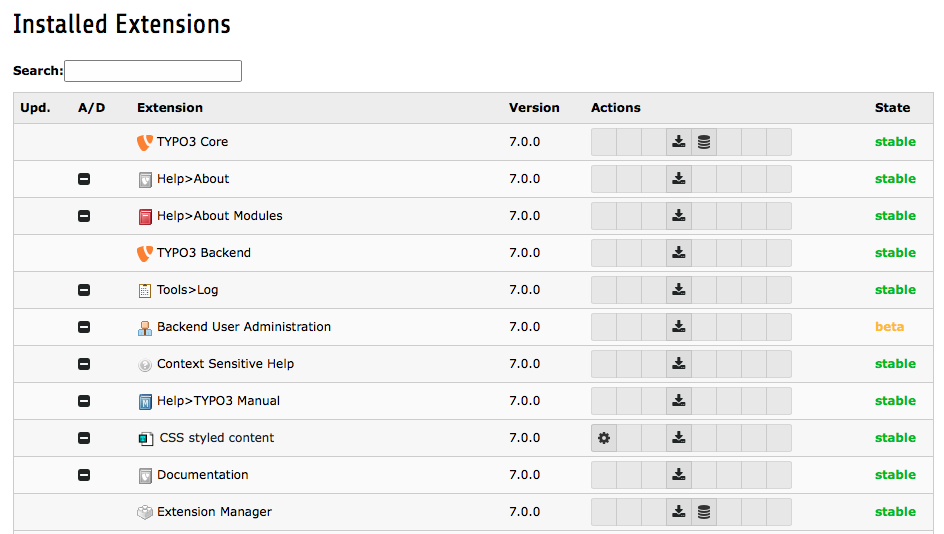
\includegraphics[width=0.99\linewidth]{BackendUserInterface/be-table.png}
	\end{figure}

\end{frame}

% ------------------------------------------------------------------------------
% LTXE-SLIDE-START
% LTXE-SLIDE-UID:		5a9c5cd3-087d936a-616b565c-02475cb1
% LTXE-SLIDE-ORIGIN:	785f717d-a7c4d1dd-f186ca6a-060c1dc4 English
% LTXE-SLIDE-TITLE:		Page And List Search
% LTXE-SLIDE-REFERENCE:	https://forge.typo3.org/issues/59763
% ------------------------------------------------------------------------------

\begin{frame}[fragile]
	\frametitle{Interfaz de usuario de Backend}
	\framesubtitle{Búsqueda en visualización de página y lista}

	\begin{itemize}
		\item Haga clic en la lupa para mostrar la barra de búsqueda en vista tipo "lista" y "página"
			(la función de búsqueda estaba al final de la página anterior)
	\end{itemize}

	\begin{figure}
		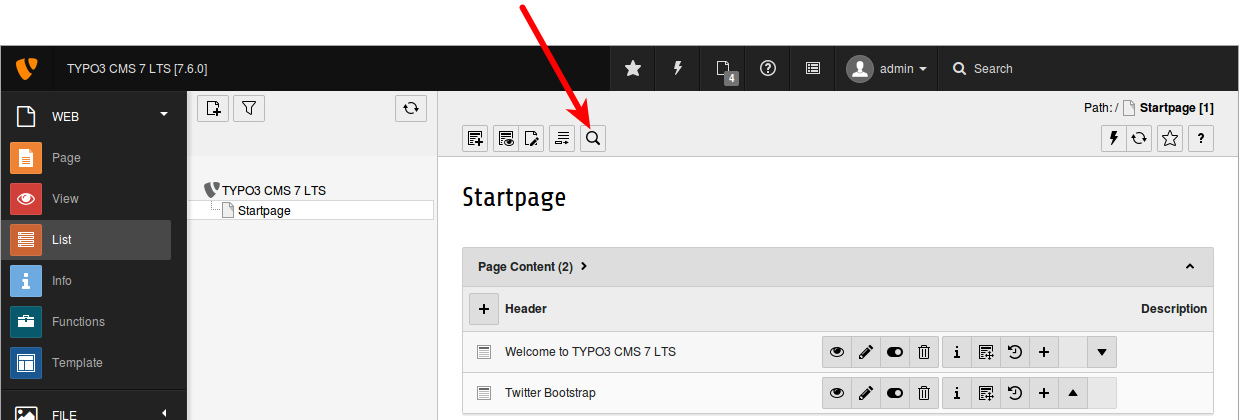
\includegraphics[width=0.95\linewidth]{BackendUserInterface/be-search.jpg}
	\end{figure}

\end{frame}

% ------------------------------------------------------------------------------
% LTXE-SLIDE-START
% LTXE-SLIDE-UID:		a6be2664-dd828239-6e4fbdb1-7fdbf1c2
% LTXE-SLIDE-ORIGIN:	df97fbbf-9ea6c6a9-d9b4c5d4-f8fe1601 English
% LTXE-SLIDE-TITLE:		Migrate Counter of Open Documents to Bootstrap "Badge"
% LTXE-SLIDE-REFERENCE:	https://forge.typo3.org/issues/61675
% ------------------------------------------------------------------------------

\begin{frame}[fragile]
	\frametitle{Interfaz de usuario de Backend}
	\framesubtitle{El distintivo muestra los documentos abiertos}

	\begin{itemize}
		\item El número de documentos abiertos se muestra como un "distintivo" Bootstrap
			(requiere extensión de sistema de "Documentos Abiertos")
	\end{itemize}
	\begin{figure}
		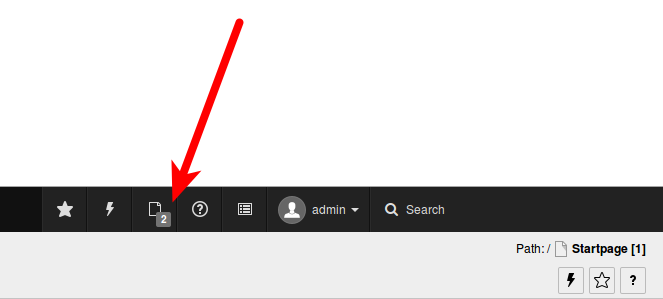
\includegraphics[width=0.75\linewidth]{BackendUserInterface/be-badge.png}
	\end{figure}

\end{frame}

% ------------------------------------------------------------------------------
% LTXE-SLIDE-START
% LTXE-SLIDE-UID:		186f5135-3b44d5ac-799a453e-48673f40
% LTXE-SLIDE-ORIGIN:	a25faae4-8c12c45e-b337b64a-0cf2f53f English
% LTXE-SLIDE-TITLE:		Rebrush FlashMessage
% LTXE-SLIDE-REFERENCE:	https://forge.typo3.org/issues/62580
% ------------------------------------------------------------------------------

\begin{frame}[fragile]
	\frametitle{Interfaz de usuario de Backend}
	\framesubtitle{Mensajes Flash}

	\begin{itemize}
		\item La apariencia visual de los Mensajes Flash ha sido actualizada
		\item Contraste de texto vs. color de fondo de casilla mejorado
	\end{itemize}

	\begin{columns}[T]
		\begin{column}{.25\textwidth}
			\smaller\hfill 
				\begingroup\color{typo3red}TYPO3 CMS < 7.0\endgroup
			\normalsize
		\end{column}

		\begin{column}{.5\textwidth}
			\begin{figure}\vspace*{-0.6cm}
				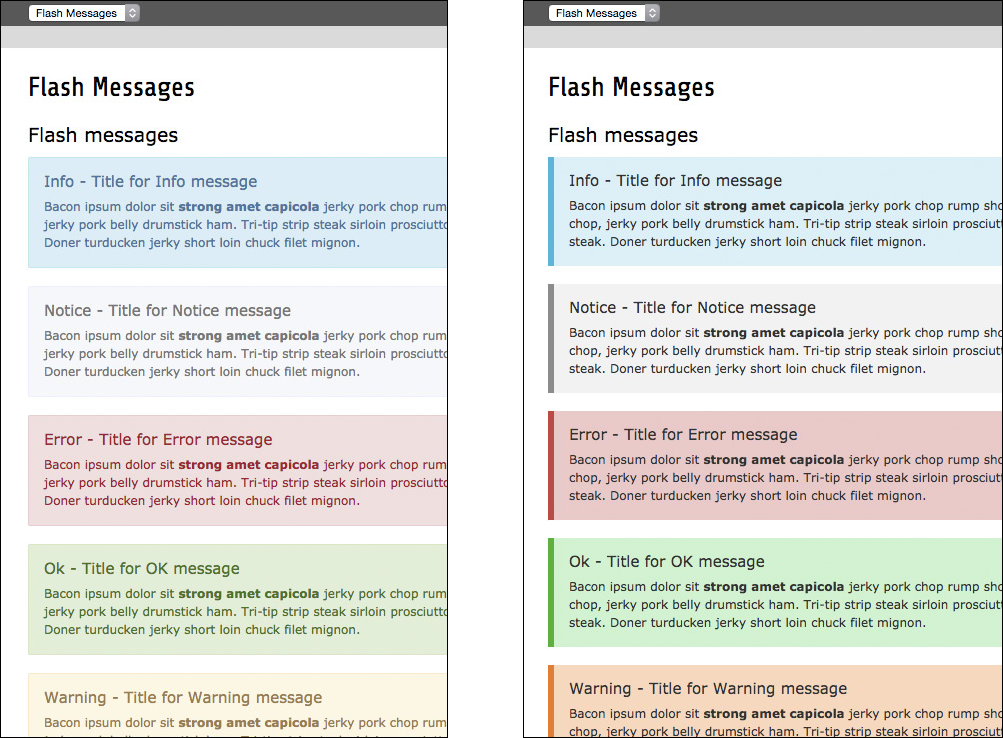
\includegraphics[width=0.99\linewidth]{BackendUserInterface/be-flashmessages.png}
			\end{figure}
		\end{column}

		\begin{column}{.25\textwidth}
			\smaller
				\begingroup\color{typo3red}TYPO3 CMS >= 7.0\endgroup
			\normalsize
		\end{column}

	\end{columns}

\end{frame}

% ------------------------------------------------------------------------------
% LTXE-SLIDE-START
% LTXE-SLIDE-UID:		ad6132c5-19cfffb5-63a2d99e-46e211fa
% LTXE-SLIDE-ORIGIN:	d6a85376-8109aa8c-45a40582-7edb975a English
% LTXE-SLIDE-TITLE:		Video Player in Info Window
% LTXE-SLIDE-REFERENCE:	https://forge.typo3.org/issues/61668
% ------------------------------------------------------------------------------

\begin{frame}[fragile]
	\frametitle{Interfaz de usuario de Backend}
	\framesubtitle{Reproductor de video en Info Windows}
	\begin{itemize}
		\item Los archivos de audio y vídeo de HTML5 pueden ser reproducidos en el info window
			(donde se muestran los metadatos)
		\begin{figure}
			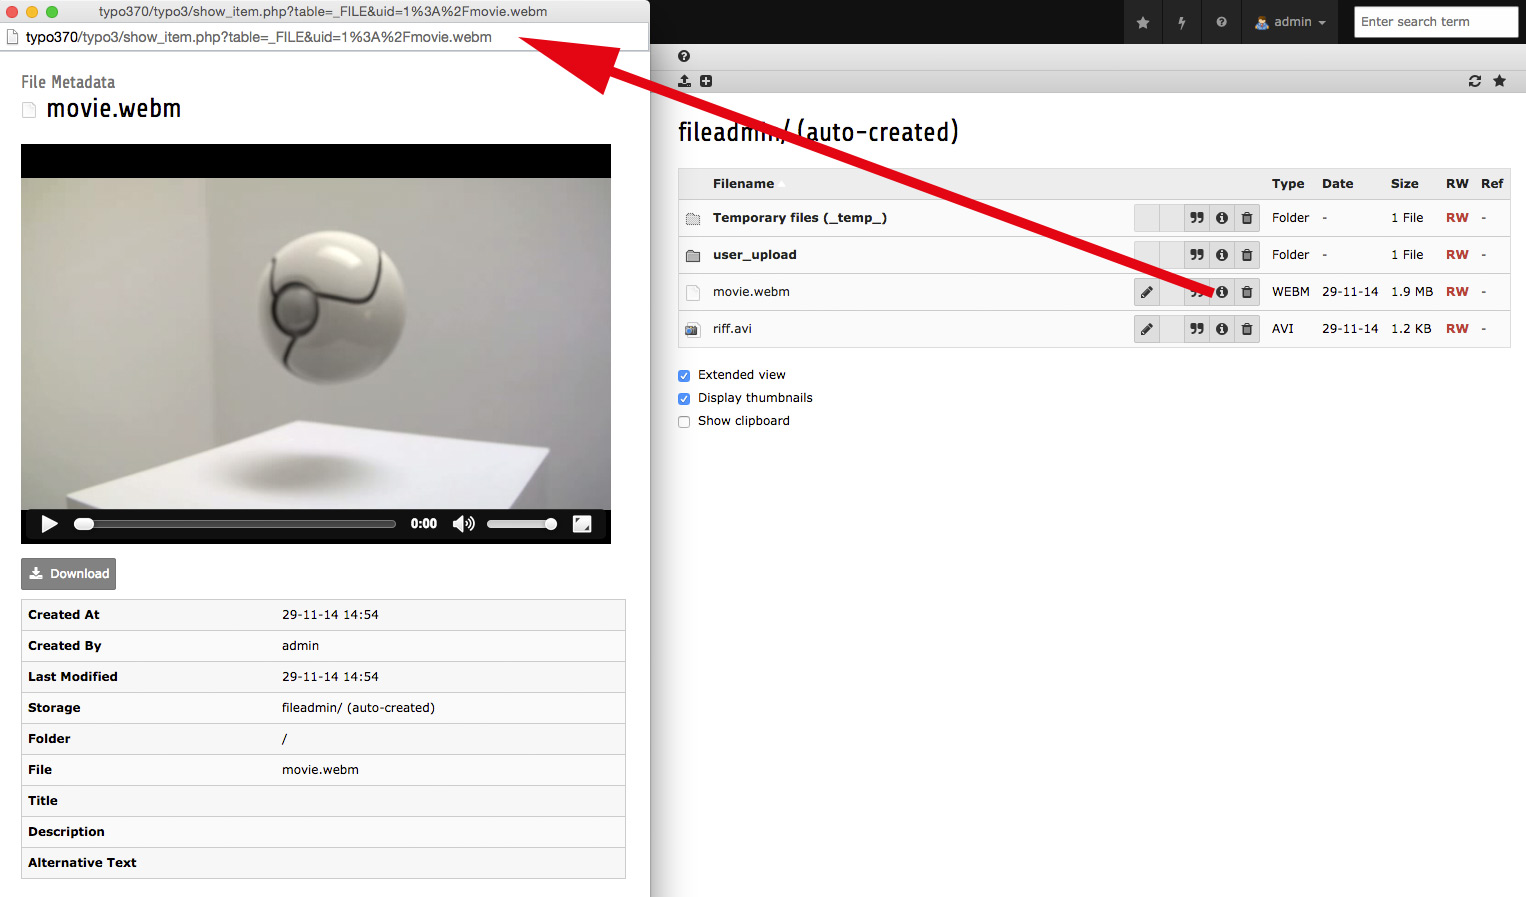
\includegraphics[width=0.70\linewidth]{BackendUserInterface/be-info.jpg}
		\end{figure}

	\end{itemize}

\end{frame}

% ------------------------------------------------------------------------------
